\documentclass[../main/Feedback.tex]{subfiles}
\begin{document}
\section{Results}
		\subsection{Mental Workload}
		\subsubsection{fNIRS data}
		A one-way repeated measures ANOVA was conducted to determine whether there was a statistically significant difference in mean Hbo values between the three web forms. The assumption of sphericity was met, as assessed by Mauchly's test of sphericity, $X^{2}(2) = 0.195, p = 0.907$. There was no significant statistical difference in the mean Hbo between the 3 web forms  $F(2,20)=3.400, p<.054,$ partial $\eta^{2}=.254$ with mean Hbo decreasing from 0.2377 (SD = 1.19) in index3 to -0.1166 (SD = 0.82) and -0.117 (SD = 1) for index2 and index1 respectfully. Which means that index3 indicates the highest workload, compared to the rest of the conditions.
		\begin{figure}[h]
			\centering
			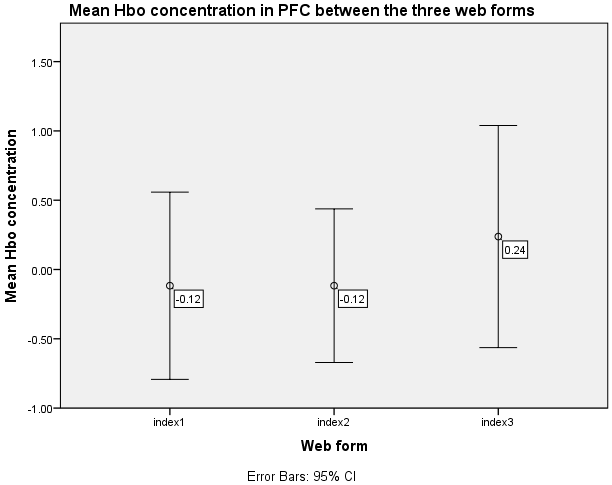
\includegraphics[width=0.7\linewidth]{mean-hbo-index123}
			\caption[mean Hbo activation between the three web forms]{Mean Hbo activation between the three web form conditions as measured by fNIRS. Higher Hbo values indicates higher mental workload experienced by the operator.}
			\label{fig:mean-hbo-index123}
		\end{figure}
		After conducting t-tests between index1 and index3 there was found a marginal statistical difference p=0.054. Which means that the measured Hbo between the two versions has a 94.6\% statistical probability that the difference are not caused by random sampling error. However, we fail to reject the first null hypothesis. This means that we could not find a statistically significant interaction, however we were very close to statistical significance, as p=0.054 and we can assume we have marginal statistical significance.
		
		\begin{figure}[h]
			\centering
			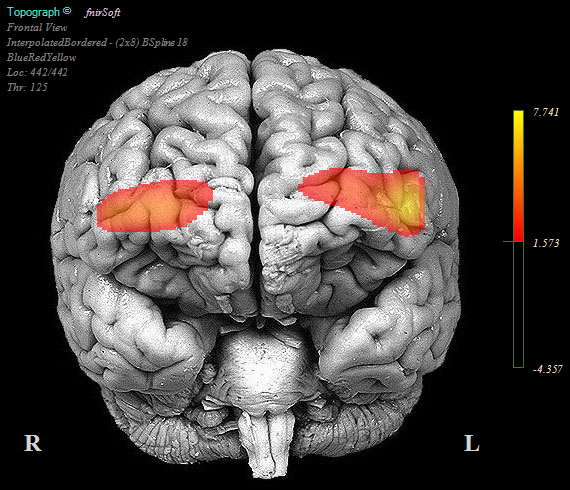
\includegraphics[width=0.7\linewidth]{p2-index3-brain-view-left-activation}
			\caption[Brain view of Participant's 2 Hbo activation during web form filling of index3]{Brain view of Participant's 2(P2) Hbo activation during web form filling of index3. It can be noted more hemodynamic activation in the left hemisphere. P2 rated its emotional valence as positive (4/5).}
			\label{fig:p2-index3-brain-view-left-activation}
		\end{figure}
		
		\begin{figure}[h]
			\centering
			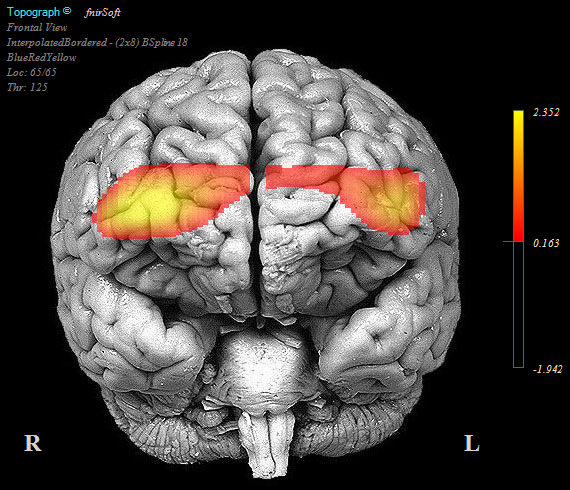
\includegraphics[width=0.7\linewidth]{p2-video3-brain-view}
			\caption[Brain view of Participant 2 while viewing video of road accident(video3)]{Brain view of Participant 2 while viewing video of road accident(video3). More arousal can be noted and more right hemisphere activation, which is expected as automotive accidents increase arrousal and emotional state becomes negative.}
			\label{fig:p2-video3-brain-view}
		\end{figure}
		Also, no statistical significance was found when comparing the means of Hbr between the three conditions $F(2,20)=2.044, p<.156,$ partial $\eta^{2}=.170$ where index2 had the highest Hbr mean 0.05 (SD = 0.85), index1 with -0.07 (SD = 0.96) and index3 with the lowest Hbr mean -0.36 (SD = 1.43). Which, accordingly negatively correlated to Hbo data, and again indicated that index3 evoke the highest workload than the other conditions. Furthermore, a repeated measures ANOVA test was conducted to elicit significant statistical differences between mean Hbt between the three web forms, however no statistical significance was found $F(2,20)=0.685, p<.516,$ partial $\eta^{2}=.064$ where index2 had the highest Hbt mean -0.08 (SD = 0.49), index3 with -0.13 (SD = 0.58) and index1 with the lowest mean Hbt -0.19 (SD = 0.49). The results indicate that Hbo was more responsive for this experiment and gave us higher significance between condition compared to Hbr and Hbt. 
		No correlation was found between the fNIRS mean data and any of the NASA-TLX scales, including the calculated total tlx. As a result, we fail to reject the second null hypothesis which states there is no difference between objective data from fNIRS and subjective data from NASA-TLX.
		\subsubsection{NASA-TLX}
		We report data for the NASA-TLX measure for all of the participants without excluding anyone because there was no problem with obtaining the data for this measure. All of the calculated data can be viewed in Table \ref{nasa-tlx}.
		There was no statistical significance between each of the NASA-TLX scales, including the total$F(2,38)=0.743, p<.482,$ partial $\eta^{2}=.038$ score as assessed by one way repeated measures ANOVA. Which means statistically we have 51.8\% chance of the results of the total NASA-TLX score to be caused by random sampling error. Also, perceived mean mental demand was lowest for index1 9.15 (SD = 4.94), index2 had slightly higher mean 9.40 (SD = 4.68) and index3 has the highest scores 10.8 (SD = 5.38). Also, mental demand had a strong positive correlation with total tlx for the 3 conditions $r(18)=0.652, p=0.002$, $r(18)=0.738, p<0.001$, and $r(18)=0.741, p<0.001$ for index1, index2 and index3 respectfully. Which supports the validity of NASA-TLX measurements. The total calculated value for the NASA-TLX was highest for index3 7.07 (SD = 3.22) decreasing to 6.92 (SD = 2.95) for index1 and 6.47 (SD = 3.11) for index2. This means that index3 requires slightly more attentional resources to complete the task compared to index1 and index2.
		There was a moderate positive correlation between mental demand scales and task completion times between the three conditions  $r(18)=0.487, p=0.030,  r(18)=0.484, p=0.030,  r(18)=0.638, p=0.002$. The results show that the more participants perceived higher workload the more their performance dropped as it took them more time to complete the task.
		
		\begin{table}[h]
			\centering
			\caption[NASA-TLX mean scores]{A table of all of the calculated mean NASA-TLX values for the 6 subscales, including the averaged total tlx}
			\label{nasa-tlx}
			\begin{tabular}{l|ccc}
				& Index1           & Index2           & Index3           \\[0.12cm]   \hline
				Mental demand   & 9.15 (SD = 4.94) & 9.40 (SD = 4.68) & 10.8 (SD = 5.38) \\
				Physical demand & 4.05 (SD = 4.08) & 2.90 (SD = 3.21) & 3.90 (SD = 3.65) \\
				Temporal demand & 7.40 (SD = 4.49)  & 7.65 (SD = 5.79) & 6.55 (SD = 4.91) \\
				Performance     & 6.65 (SD = 3.79) & 5.60 (SD = 3.62)  & 6.20 (SD = 3.86)  \\
				Effort          & 8.15 (SD = 4.58) & 7.35 (SD = 4.68) & 8.20 (SD = 5.30)   \\
				Frustration     & 6.10 (SD = 5.11)  & 6.00 (SD = 3.66)  & 6.75 (SD = 5.22) \\\hline
				Total 			& 6.92 (SD = 2.95) & 6.47 (SD = 3.11) & 7.07 (SD = 3.22)
			\end{tabular}
		\end{table}
		
		\subsubsection{SAM - arousal scale}
		As it can be seen from Figure~\ref{fig:sam-arrousal-index123} the perceived arousal was lowest for index1 2.8 (SD = 0.95) increasing to 2.95 (SD = 1.05) for index2 and to 3.15 (SD = 1.18) for index3 respectfully. No statistical significance was found when comparing the means between the three conditions $F(2,38)=2.462, p<0.099$ partial $\eta^{2}=.115$ using one way repeated measures ANOVA. However, after running post hoc test without adjustments(LSD) a statistically significant difference was found between index1 and index3 $p=0.049$. Which means that perceived arousal was significantly higher for index3 compared to index1.
		Also, the time to complete index1 and index2 positively correlated to perceived arousal for index 1 and index2:$r(18)=0.551, p=0.012$ and $r(18)=0.473, p=0.035$. However time to complete index3 does not correlate to perceived arousal of index3 $r(18)=0.269, p=0.252$. Which indicates that we have a partial positive correlation between the perceived arousal, which can be considered as workload, for the web forms and the time to complete them.
		
		\begin{figure}[h]
			\centering
			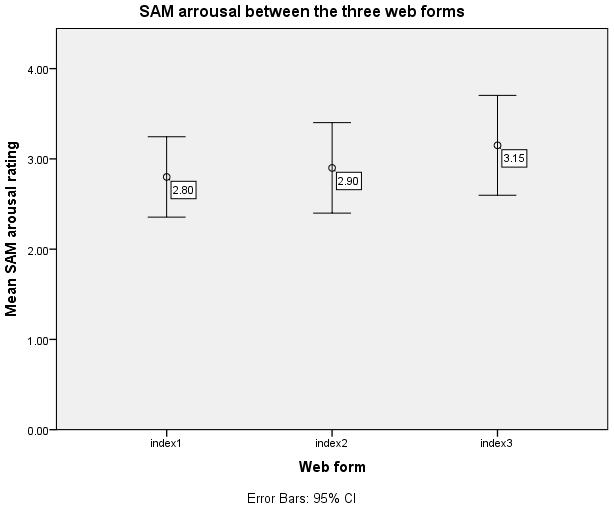
\includegraphics[width=0.7\linewidth]{sam-arrousal-index123}
			\caption[SAM arrousal between the three web forms]{The mean SAM arrousal rating obtained from the three web form conditions.}
			\label{fig:sam-arrousal-index123}
		\end{figure}
		
		\subsection{Emotional Valence}
		\subsubsection{fNIRS differences}
		\paragraph{Data from the period of web form filling}\leavevmode\\
		\begin{figure}[h]
			\centering
			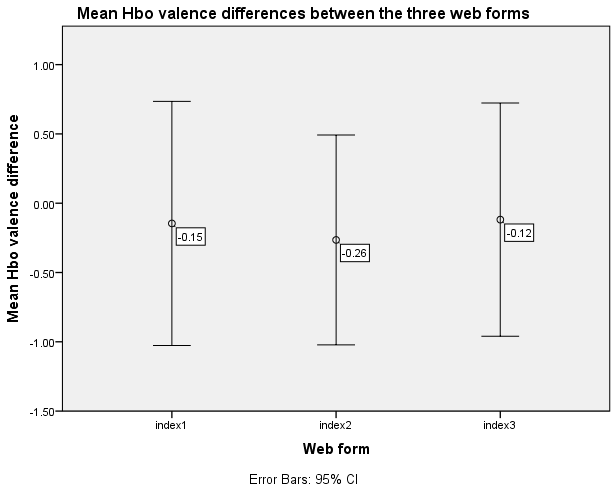
\includegraphics[width=0.7\linewidth]{hbo-valence-differences-index123}
			\caption[Hbo valence differences between the three web forms]{The mean Hbo valence differences obtained from the fNIRS for the three web form conditions. Higher values indicate more positive affect, and lower value more negative affect.}
			\label{fig:hbo-valence-differences-index123}
		\end{figure}									
		To begin with, Figure \ref{fig:hbo-valence-differences-index123} shows the valence differences in Hbo concentration between the left and right hemispheres. fNIRS Hbo valence differences was highest for index3 -0.12 (SD = 1.25) decreasing to -0.15 (SD = 1.31) for index1 and the lowest value was for index2 -0.26 (SD = 1.13). Indicating that participants experienced the most positive when completing the index3 condition, slightly less positive for index1 and the least positive when completing index2. However significant statistical difference was not found $F(2,20)=0.392, p<0.681,$ partial $\eta^{2}=.038$ as assessed by one-way repeated measures ANOVA.
		
		The Hbr valence differences were highest for index2 0.34 (SD = 1.18) decreasing to 0.18 (SD = 1.39) for index3 and to 0.10 (SD = 1.68) for index1. Signifying that index2 elicited the most negative affect compared to the rest of the conditions. However, the difference was not statistically significant.
		The Hbt mean valence difference values for index1 were lower -0.45 (SD = 0.79) compared to index2 0.06 (SD = 0.56) and index3 0.05 (SD = 0.87) respectfully. There was no statistical significance as assessed by one way repeated measures ANOVA between the three conditions for Hbr valence differences: $F(2,20)=0.418, p<0.664,$ partial $\eta^{2}=.040$ and Hbt valence differences: $F(2,20)=0.302, p<0.743,$ partial $\eta^{2}=.029$. Also, there was strong positive correlation between temporal NASA-TLX scale of index1 and the Hbo valence differences of index1 $r(9)=0.766, p=0.006$, however, there was no correlation found between index2: $r(9)=0.581, p=0.061$ and index3: $r(9)=0.218, p=0.519$ which suggests that as participants perceived more temporal demand the obtained mean Hbo data increased.\\
		
		\paragraph{Data from the period of video clips}\leavevmode\\
		The mean Hbo valence difference for video3 was the highest with 0.17 (SD= 0.25) compared to video1 with -0.01 (SD = 1.32) and video2 with -0.8 (SD = 1.20), suggesting that participants experienced more positive emotion when watching video3 compared to video1 and video2. In contrast, mean Hbr valence difference values for video3 were the lowest with -0.25 (SD = 0.47) compared to video1 0.30 (SD = 1.20) and video2 0.32 (SD = 0.89). For the mean Hbt valence difference values video1 was the highest with 0.18 (SD = 0.71) decreasing to 0.07 (SD = 0.64) for video3 and to -0.06 (SD = 0.35) for video2.\\
		A one-way repeated measures ANOVA was conducted to determine whether there was a statistically significant difference in Hbo, Hbr and Hbt valence differences between the three videos. There was no significant statistical difference in the mean Hbo valence difference between the 3 videos $F(2,20)=0.051, p<0.951,$ partial $\eta^{2}=.005$, the mean Hbr valence difference: $F(2,20)=0.062, p<0.940,$ partial $\eta^{2}=.006$ and the mean Hbt valence difference: $F(2,20)=0.522, p<0.601,$ partial $\eta^{2}=.050$. Consequently, we cannot find significant difference in the emotional valence from the objective data between the three videos.
		There was no correlation found between Hbo valence differences and SAM emotional valence subjective scale for the three videos $r(9)=-0.490, p=0.126$; $r(9)=0.095, p=0.781$; $r(9)=0.496, p=0.121$. As a result, we fail to reject the third null hypothesis, which states that there is no correlation between the fNIRS valence difference data and the SAM subjective scale of emotional valence.
		
		\subsubsection{SAM emotional valence}
		\paragraph{Data from the period of web form filling}\leavevmode\\
		The perceived mean emotional valence for index1 was the lowest with 
		3.1 (SD = 0.97) increasing to 3.4 (SD = 0.99) for index2 and to 3.7 (SD = 0.98) for index3, as it can be seen from Figure \ref{fig:sam-valence-index123}.
		\begin{figure}[h]
			\centering
			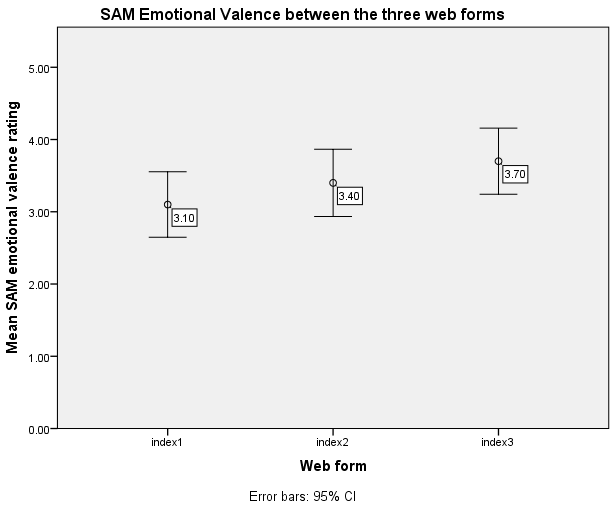
\includegraphics[width=0.7\linewidth]{sam-valence-index123}
			\caption[emotional valence between the 3 conditions]{Perceived emotional valence between the 3 web form conditions}
			\label{fig:sam-valence-index123}
		\end{figure}
		A one-way repeated measures ANOVA was conducted to determine whether there was a statistically significant difference in SAM emotional valence scale values between the three web forms. The assumption of sphericity was met, as assessed by Mauchly's test of sphericity, $X^{2}(2) = 0.446, p = 0.800$. There was no significant statistical difference in the SAM emotional valence scale between the 3 web forms  $F(2,38)=2.803, p<.073,$ partial $\eta^{2}=0.129$ with mean SAM emotional valence increasing from 3.1$\pm$0.97 in index1 to 3.4$\pm$0.99 and 3.7$\pm$0.98 for index2 and index3 respectfully. This means we cannot distinguish which web form participants perceived as more positive or negative, however we had marginal statistical significance which gives us high probability that the results were not being biased by random sampling error.	
		
		\paragraph{Data from the period of video clips}\leavevmode\\
		The perceived mean emotional valence for video3 was the highest with 3.1 (SD = 1.07) decreasing to 2.9 (SD = 1.33) for video1, and 2.7 (SD = 0.98) for video3. There was no statistical significance as assessed by one way repeated measures ANOVA between the three videos for SAM emotional valence: $F(2,38)=0.792, p<0.460,$ partial $\eta^{2}=.040$. The data suggest that we cannot compare the perceived emotional valence between the 3 video due to high chance of the results being caused by random sampling error.
		\subsection{User performance and preferences}
		\subsubsection{Task completion time}		
		\begin{figure}[h]
			\centering
			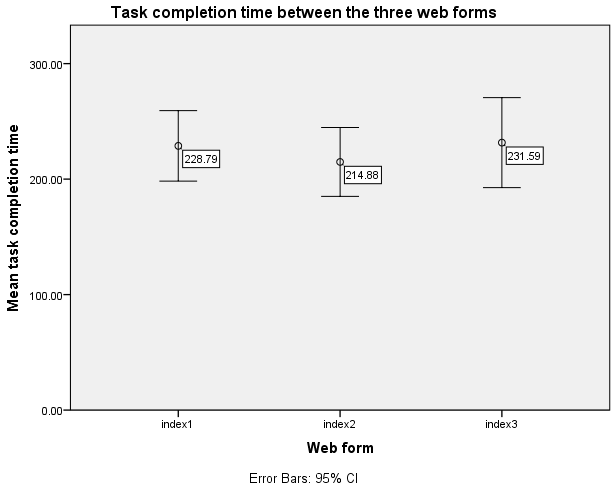
\includegraphics[width=0.85\linewidth]{mean-task-completion-time}
			\caption[Task completion time between the three web forms]{Mean task completion time between the three web forms}
			\label{fig:mean-task-completion-time}
		\end{figure}
		It can be seen from Figure \ref{fig:mean-task-completion-time} that the mean time to complete index2 was the lowest 214.88 (SD = 63.81) increasing to 228.79 (SD = 65.19) for index1 and to 231.60 (SD = 83.33) for index3. However, there was no significant statistical difference in time to complete between the 3 web forms $F(2,38)=0.556, p<.578,$ partial $\eta^{2}=.028$, as assessed by one-way repeated measures ANOVA. The results indicate that the performance was lowest when participants completed index3, slightly higher for index1 and the highest for index2.
		Also, the time to complete index2 and index3 had a strong positive correlation with perceived effort(NASA-TLX) for index2 and index3: $r(18)=0.702, p=0.016$ and $r(18)=0.634, p=0.036$. However, time to complete index1 does not correlate to perceived effort of index1 $r(18)=0.216, p=0.524$. This suggests that when participants perceived more effort it took them more time to complete the web form.
		\subsubsection{User preferences from the short-interview question}
		
		After the end of the experiment participants were asked which of the three web forms they prefer the most which is depicted in Figure \ref{fig:user-preferences}. The bulk of them preferred index3 and index1 with 10 and 9 votes respectively compared to index2 which was only preferred by 3 participants. user-prefe The given answer were transcribed as can be seen in Appendix \ref{App:AppendixD}.
		\begin{figure}[h]
			\centering
			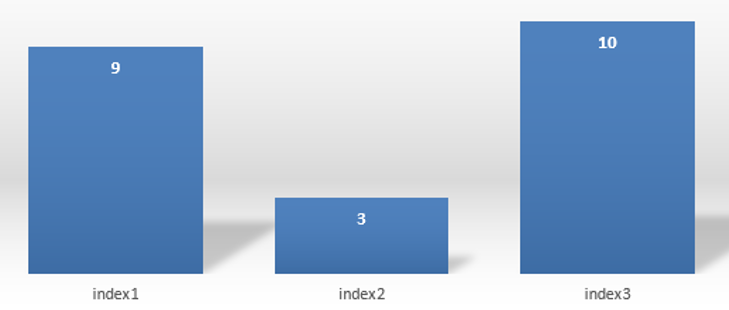
\includegraphics[width=0.7\linewidth]{user-preferences}
			\caption[Participant preferences]{At the end of the experiements participants were asked which of the 3 web forms they preferred the most. Th sum of the amswers is depicted in a bar chart.}
			\label{fig:user-preferences}
		\end{figure}			 
\section{Conclusions}

\end{document} 